\section{System Description}
\label{sec:system}

The Piping and Instrumentation Diagram (P\&ID) of the three stages
of the systems is shown in Fig.~\ref{fig:PID}.

% ----------------------------------------------------------
\begin{figure}[h]
    \centering
    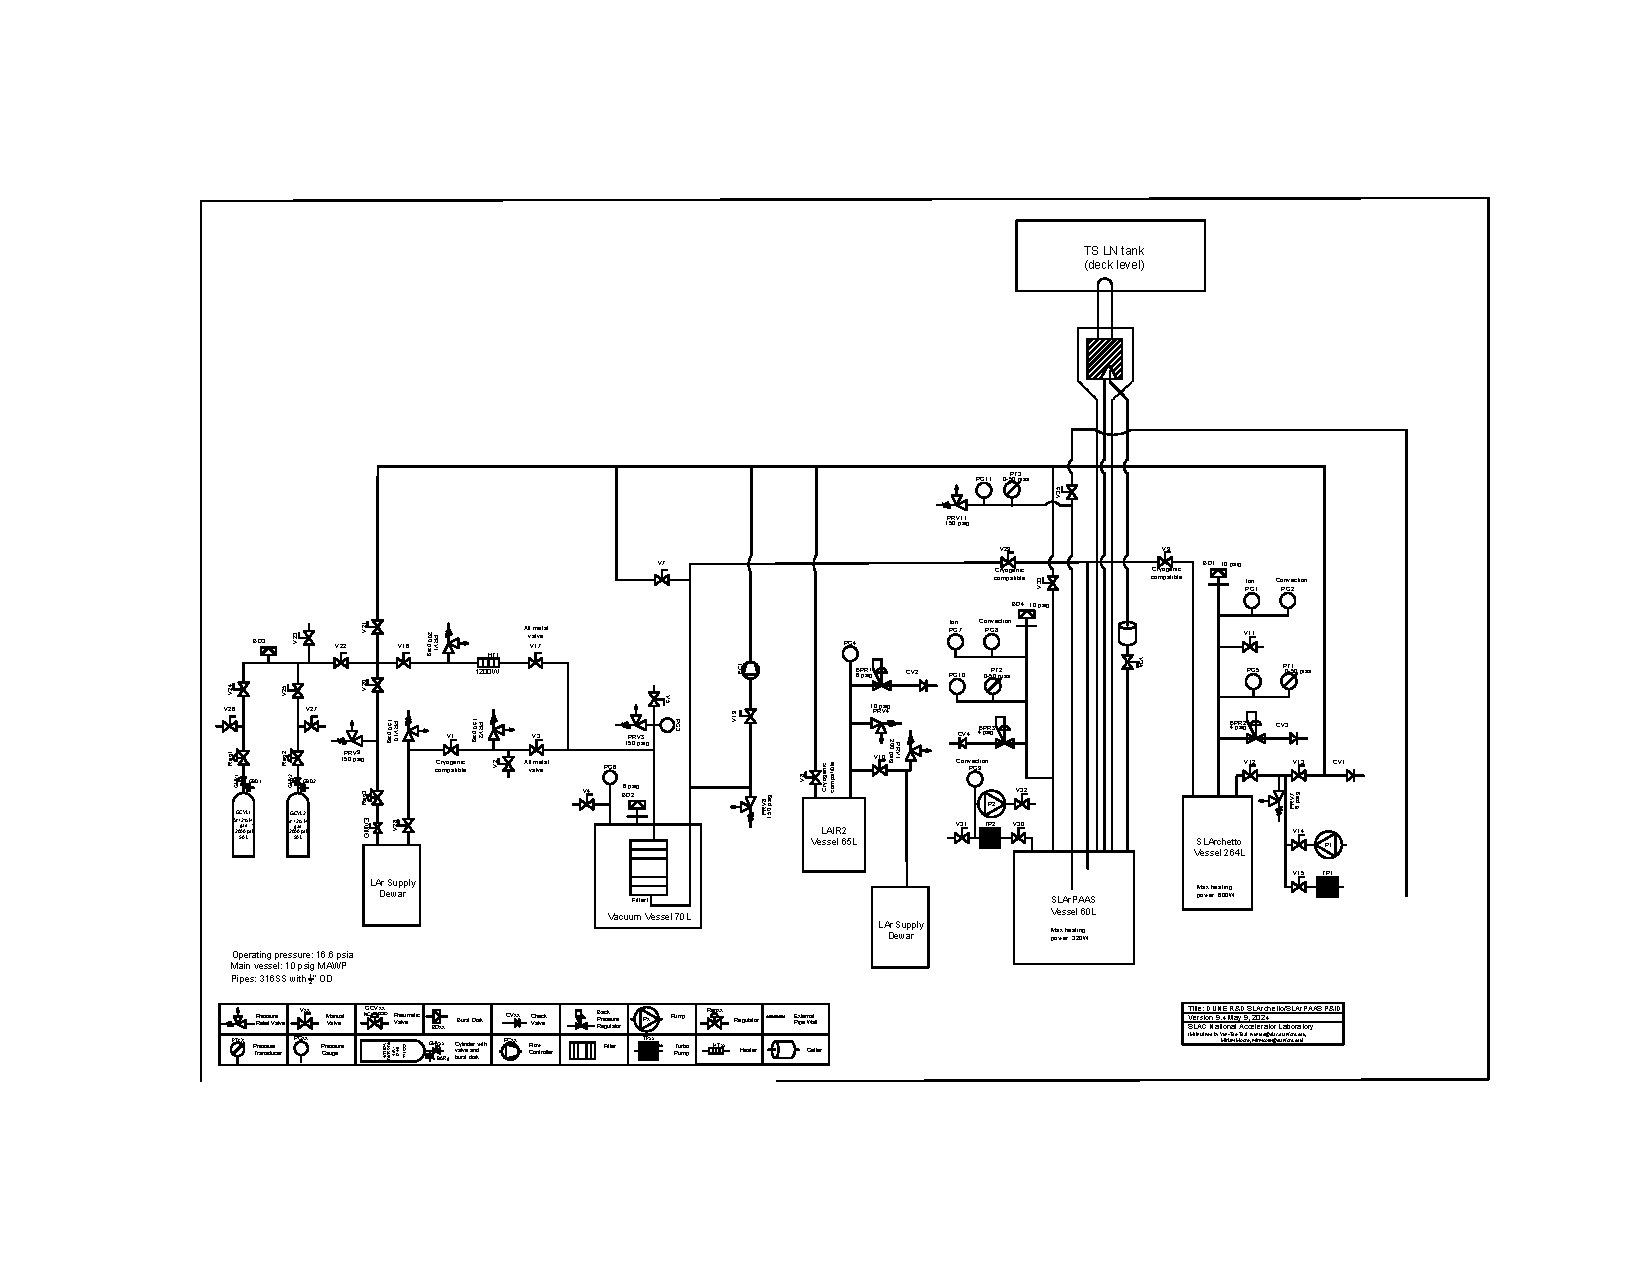
\includegraphics[width=\textwidth]{fig/PID_SLArchettoPAAS_v9.4.pdf}
    \caption{P\&ID of the LAr setups at LNTF.}
    \label{fig:PID}
\end{figure}
% ----------------------------------------------------------

\begin{enumerate}
    \item The SLArpaas I Main Dewar (App.~\ref{app:dewar_drawing}) is a vacuum jacketed 
    vessel made by Cryofab. Vendor part number is CF1424.
    It is constructed using stainless steel 304 with an inner diameter of 13.9" 
    and inner wall thickness of 0.024". 
    The vendor states that it has a maximum allowable working pressure (MAWP) 
    of 10~psig (24.7~psid), as indicated in App.~\ref{app:mawp_statement}.
    \item The top plate (App.~\ref{app:top_plate_drawing}) of the dewar has a design 
    pressure of 12.5~psig. 
    The top plate of the dewar was designed by SLAC and built by Kurt J. Lesker.
    The thickness is 0.5" and the diameter is 18". 
    The top plate has 7~ports in it made from tubing and CF Nipple Flanges. 
    These are for piping and components. All components have the MAWP at 10~psig or higher.
    \item The SLArpaas I system consists of the Main Dewar, piping, valves, pressure gauges, 
    several pressure relief valves, a back pressure regulator, and a burst disc. 
    The part list can be found at 
    \url{https://docs.google.com/spreadsheets/d/11fEcZshcpTCyHwYS0NZCCt5l-Bi3EURLQWpjkcul8r0/edit?usp=sharing}. 
    The entire Bill of Materials is listed in a spreadsheet in the package. 
    The burst disc, which is connected to the top plate of the main dewar, 
    has a nominal cracking pressure of 10~psig, the same as the MAWP of the dewar. 
    This burst disc has a discharge capacity of 435~scfm, sufficient to prevent the dewar 
    from over-pressurizing and exploding if exposed the worst-case scenario of an external fire. 
    The discharge flowrate at different scenarios including the fire condition was calculated. 
    See Sec.~\ref{sec:discharge_rate} below for the details. 
    Refer to App.~\ref{app:manufacturer} for Product Literature including the burst disc.
    \item The normal working pressure is 1--3~psig. 
    The Main Dewar is a vacuum jacketed vessel, but the top plate is not insulated. 
    % To prevent the dewar seeing a pressure closer to the cracking pressure of the burst disc, 
    A back pressure regulator (BPR3) set to 4~psig is used to regulate the pressure in the Main Dewar.
    % The BPR3 will open when the inlet pressure reaches 6 psig and reseal when the pressure reduces to less than 6 psig. 
    The check valve (CV4) at the outlet of the BPR3 prevents back streaming, and will open
    at 1~psid. 
    The BPR3 has a flow coefficient of 0.2, which is sufficient to regulate the pressure to 
    be not higher than 4~psig at the dewar. 
    Refer to App.~\ref{app:manufacturer} for Product Literature including the BPR.
\end{enumerate}
